\documentclass{article}
\usepackage[margin = .7in]{geometry}
\usepackage[dvipdfmx]{graphicx}
\usepackage{listings}
\usepackage{amsmath}
\usepackage{bm}
\lstset{%
  language={python},
  basicstyle={\small},%
  identifierstyle={\small},%
  commentstyle={\small\itshape},%
  keywordstyle={\small\bfseries},%
  ndkeywordstyle={\small},%
  stringstyle={\small\ttfamily},
  frame={tb},
  breaklines=true,
  columns=[l]{fullflexible},%
  numbers=left,%
  xrightmargin=0zw,%
  xleftmargin=3zw,%
  numberstyle={\scriptsize},%
  stepnumber=1,
  numbersep=1zw,%
  lineskip=-0.5ex%
}

\begin{document}
\title{STAT6011/7611/6111/3317 \\ 
COMPUTATIONAL STATISTICS (2016 Fall) \\
Assignment 3}
\author{Kei Ikegami (u3535947)}
\maketitle

\section{}
	\subsection{}
		\begin{align*}
			p({\bf y} | \sigma^2) &= \idotsint \Pi_{i = 1}^{n} \frac{1}{\sqrt{2\pi}} \exp\left( -\frac{(y_i - \theta_i)^2}{2}\right)\frac{1}{\sqrt{2\pi}\sigma} \exp\left( -\frac{\theta_i^2}{2\sigma^2}\right)\mathrm{d}\theta_1 \dots \mathrm{d}\theta_n \\
			&= \idotsint \Pi_{i = 1}^{n} \frac{1}{\sqrt{2\pi}\sqrt{\sigma^2 + 1}} \exp\left( -\frac{y_i}{2} + \frac{\sigma^2 y_i^2}{2(\sigma^2 + 1)}\right) \frac{\sqrt{\sigma^2 + 1}}{\sqrt{2\pi}\sigma} \exp\left( \frac{\sigma^2 + 1}{\sigma^2} \left(\theta_i -\frac{\sigma^2}{\sigma^2 + 1}y_i \right)\right)\mathrm{d}\theta_1 \dots \mathrm{d}\theta_n \\
			&= \Pi_{i = 1}^{n} \frac{1}{\sqrt{2\pi}\sqrt{\sigma^2 + 1}} \exp\left( -\frac{y_i}{2} + \frac{\sigma^2 y_i^2}{2(\sigma^2 + 1)}\right) \\
			&= \left(\frac{1}{\sqrt{2\pi}\sqrt{\sigma^2 + 1}}\right)^{n} \exp \left( -\frac{\sum_{i=1}^{n} y_i}{2} + \frac{\sigma^2 \sum_{i=1}^{n} y_i^2}{2(\sigma^2 + 1)}\right)
		\end{align*}
	\subsection{}
		\begin{align*}
			p(\sigma^2 | {\bf y}) \propto \left(\frac{1}{\sqrt{2\pi}\sqrt{\sigma^2 + 1}}\right)^{n} \exp \left( -\frac{\sum_{i=1}^{n} y_i}{2} + \frac{\sigma^2 \sum_{i=1}^{n} y_i^2}{2(\sigma^2 + 1)}\right) \frac{1}{\sigma^2}
		\end{align*}
		\lstinputlisting[caption=1-b]{1-b.py}
		\begin{center}
		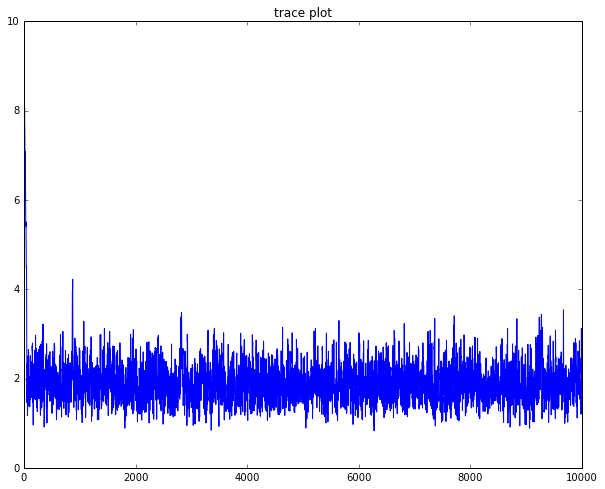
\includegraphics[width = 12cm]{1-b.png}
		\end{center}
	\subsection{}
	Let $\Theta = (\theta_1, \theta_2, \dots , \theta_n)$, and let $\Theta_{-j} = (\theta_1, \dots, \theta_{j-1}, \theta_{j+1}, \dots, \theta_n)$.
		\begin{align*}
			p(\sigma^2 | {\bf y}, \Theta) &\propto \frac{1}{\sigma^2(\sqrt{2\pi \sigma^2})^n} \exp\left( -\frac{\sum_i^n \theta_i^2}{2\sigma^2}\right) \\
			p(\theta_j | {\bf y}, \Theta_{-j}, \sigma^2) &\propto N \left( \frac{\sigma^2 y_j}{\sigma^2 + 1}, \frac{\sigma^2}{\sigma^2 + 1}\right) \forall j \in \left\{1, 2, 3, \dots, n \right\} \\
		\end{align*}
		\lstinputlisting[caption=1-c]{1-c.py}
		Trace plot. $\sigma^2$ and $\theta_1$.
		
		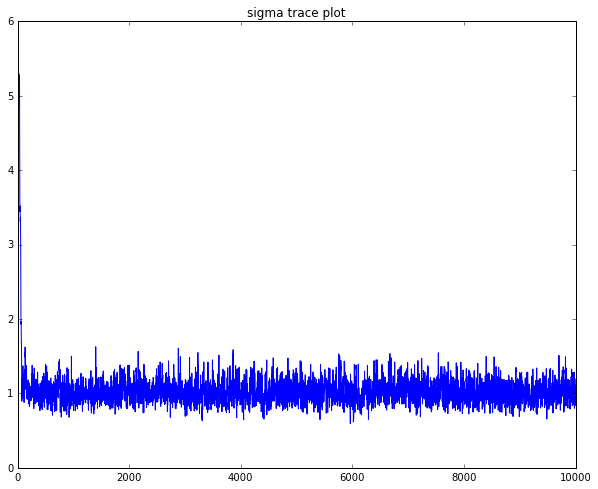
\includegraphics[width = 9cm]{1-c-sigma.png}
		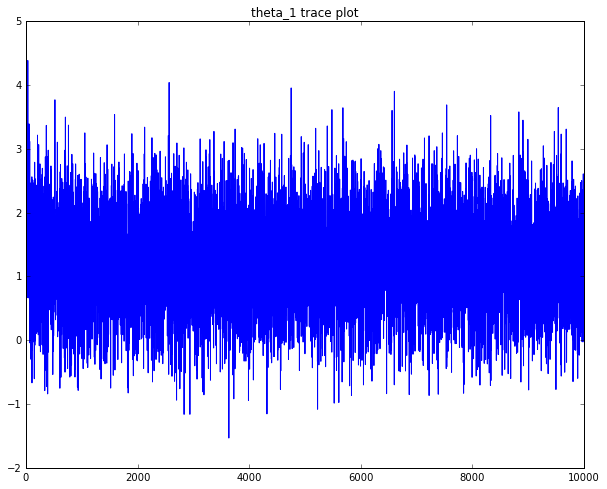
\includegraphics[width = 9cm]{1-c-theta.png}
		
	
\section{}
	\subsection{}
	\subsection{}
	\subsection{}
	\subsection{}

\section{}
	\subsection{}
	\subsection{}
	
	
	
	
	
	
\end{document}